\documentclass[a4paper, 12pt]{article}%тип документа

%отступы
\usepackage[left=2cm,right=2cm,top=2cm,bottom=3cm,bindingoffset=0cm]{geometry}

%Русский язык
\usepackage[T2A]{fontenc} %кодировка
\usepackage[utf8]{inputenc} %кодировка исходного кода
\usepackage[english,russian]{babel} %локализация и переносы

%Вставка картинок
\usepackage{graphicx}
\graphicspath{{pictures/}}
\DeclareGraphicsExtensions{.pdf,.png,.jpg}

%Графики
\usepackage{pgfplots}
\pgfplotsset{compat=1.9}

%Математика
\usepackage{amsmath, amsfonts, amssymb, amsthm, mathtools}

%Заголовок
\author{Талашкевич Даниил Александрович \\
группа Б01-009}
\title{Работа 1.3.1 \\
Определение модуля Юнга на основе исследования деформаций растяжения и изгиба}
\begin{document}
\maketitle
\newpage
\textbf{Цель работы:} экспериментально получить зависимость между напряжением и деформацией (закон Гука) для двух простейших напряженных состояний упругих тел: одноосного растяжения и чистого изгиба; по результатам измерений вычислить модуль Юнга. \\
\textbf{В работе используется:} прибор лермантова, проволока из исследуемого материала, зрительная трубка со шкалой, набор грузов, микрометр, рулетка; во второй части - стойка для изгибания балки, индикатор для измерения величины прогиба, набор исследуемых стержней, грузы, линейка, штангенциркуль.
\begin{center}
{\section{I. Определение модуля Юнга по измерениям растяжения проволоки}}
\end{center}

Для определения модуля Юнга будем использовать прибор Лермантова, схема которого изображена на рис. 1. Верхний конец проволоки П, изготовленной из исследуемого материала, прикреплен к консоли К, а нижний -- к цилиндру, которым оканчивается шарнирный кронштейн Ш. На этот же цилиндр опирается рычаг $r$, связанный с зеркальцем З. Таким образом, удлинение проволоки можно измерить по углу ворота зеркальца.

Натяжение проволоки можноменять, перекладывая грузы с площадки М на плоащдку О и наоборот. Такая система позволяет исключить влияние деформации кронштейна К на точность измерений, так как нагрузка на нем все время остается постоянной.

При проведении эксперимента следует иметь в виду, что проволока П при отсутствии нагрузки всегда несколько изогнута, что не может не сказаться на результатах, особенно при небольших нагрузках. Проволока вначале не стлько растягивается, сколько распрямляется.


\section{Ход работы}


\subsection{Определение площади поперечного сечения проволоки.}

Определим площадь поперечного сечения проволоки. Для этого измерим ее диаметр микрометром не менее чем в десяти местах и во взаимно перпендикулярных направлениях в каждом месте. При измерении следите, чтобы микрометр не деформировал проволоку. В дальнейших расчетах надо пользоваться средним значением диаметра, вычисленным по всем измерениям.

\begin{enumerate}
\item Меряем $d$.
\item Измеряем площадь поперечного сечения проволоки
\[S =\dfrac{ \pi (\overline{d})^2}{4}.\]
\[\sigma_S = S\sqrt{2\left( \dfrac{\sigma_d}{d}\right) ^2}.\]

\item Тогда окончательно имеем:
\[S = (S \pm\sigma_S) \text{ мм}^2\]
\end{enumerate}

\subsection{Длина проволоки}

Измерим длину проволоки.

\begin{enumerate}
\item Измеряем длинну проволоки $l$
\item Направляем зрительную трубу на зеркальце так, чтобы мы четко видели шкалу, тогда свет от шкалы будет падать примерно перпендикулярно шкале на зеркало, поэтому
\[\Delta l =\dfrac{nr}{2h}\]
\[ \sigma_{\Delta l} = \Delta l\sqrt{\left( \dfrac{\sigma_{n}}{n}\right)^2 + \left(\dfrac{\sigma_d}{d}\right)^2+\left(\dfrac{\sigma_h}{h}\right)^2} \]
\end{enumerate}

\subsection{Измерение $h$, вывод формул}

Направим зрительную трубу на зеркальце З. При этом в трубу должно быть четко видно отражение шкалы в зеркальце. Формулу, связывающую число делений по шкале $n$, расстояние $h$ от шкалы до зеркальца, длины рычага $r$ и удлинение проволоки $\Delta l$, выведим самостоятельно. Длна рычага $r$ указана на приборе, а расстояние измерим сами.

\begin{enumerate}

\item где $r$ см - длина рычага, разница показаний шкалы - $n$, расстояние от шкалы до проволоки - $h$.

\end{enumerate}

\subsection{Определение максимальной величины нагрузки}

Необходимо позаботиться о том, чтобы в процессе эксперимента не выйти за пределы области, где удлинение проволоки пропорционально ее натяжению (область пропорциональности). Для этого прежде всего оценим максимальную величину нагрузки, пирняв, что разрушающее напряжение равно $900 \frac{H}{\text{мм}^2}$. Рабочее напряжение не должно превышать $30 \%$ от величины разрушающего. Проверим правильность сделанной оценки. Для этого нагрузим проволоку одним из имеющихся шрузов, затем уберем его и посмотрим, вернулась ли длина проволоки к первоначальному значению. Повторим этот эксперимент с двумя, тремя и т.д. грузами, постепенно доходя до расчетной нагрузки. Если остаточные деформации станут заметными, дальнейее увеличение нагрузкиследует прекратить. При изменении нагрузки на проволоке каждый раз необходимо предварительно арретировать прибор (на рис.1 арретир на показан).

\begin{enumerate}
\item Исходя из того, что $\sigma_{\text{предел}} = 900 \text{ Н}/\text{мм}^2$ получаем, что предельный вес, который можно повесить, чтобы не выйти за пределы $P_{\text{предел}} = 0,3 \sigma_{\text{предел}} S$. 
\end{enumerate}

\subsection{Зависимость удлинения проволоки}

Снимим зависимость удлинения проволоки, то есть числа делений $n$ по шкале, от массы грузов $m$ при увеличении и уменьшении нагрузки. Повторим этот эксперимент 2--3 раза.

\begin{enumerate}
\item Снимем зависимость удлинения проволоки от массы грузов при увеличении и уменьшении нагрузки 2-3 раза 
\end{enumerate}

\subsection{График зависимости удлинения проволоки $\Delta l $ от нагрузки $P$}

По полученным данным построим график зависимости удлинения проволоки $\Delta l $ от нагрузки $P$. В недеформированном состоянии проволока, как правилоЮ изогнута, и при малых нагрузках ее <<удлинение>> определяется не растяжением, а выпрямлением. Поэтому на начальном участке зависимости $\Delta l (P)$ (при малых $P$) удлинение растет довольно быстро, и только затем точки начинают ложиться на прямую, не проходящую, однако, через начало координат. По наклону этой прямой можно определить жесткость проволоки $k$, а по ней -- модуль Юнга. Начальный участок зависимости $\Delta l (P)$ из обработки следует исключить.

\begin{enumerate}
\item Построим график зависимости удлинения проволоки от нагрузки. В недеформированном состоянии проволока, как правило, изогнута, и при малых нагрузках её "удлинение" определяется не растяжением, а выпрямлением. Найдем уравнение получившийся прямой по МНК. По наклону прямой определим жесткость проволоки, а по ней - модуль Юнга. Начальный участок графика при обработке следует исключить. 
\end{enumerate}


\subsection{Модуль Юнга}

По найденным графически жесткости проволоки $k$ определим модуль Юнга $E$. Оценим погрешность определния $k$ $E$.

\begin{enumerate}
\item По найденной графически жёсткости проволоки найдем модуль Юнга по формуле
\[E = \dfrac{k*l_0}{S}\]
\[\sigma_E = \sqrt{\left( \dfrac{\sigma_{k}}{k} \right)^2 + \left( \dfrac{\sigma_{S}}{S} \right)^2 + \left( \dfrac{\sigma_{l_0}}{l_0} \right)^2 }\]
\end{enumerate}

\subsection{Определения материала}

Определим материал проволоки, сравнивая полученное значение модуля Юнга с табличным значениями.

\begin{enumerate}
\item Исходя из полученных данных определяем материал.
\end{enumerate}
\section{II. Определение модуля Юнга по измерениям изгиба балки}

Экспериментальная установка состоит из прочной стойки с опорными А и Б (рис.2). На ребра призм опирается исследуемый стержень (балка) В. В середине стежня на призме Д подвешена площадка П с грузами. Измерять стрелу прогиба можно с помощью индикатора И, укрепляемого на отдельной штанге. Полный оборот большой стрелки индикатора соответствует 1 мм и одному делению малого циферблата.

\begin{figure}[h]
\center{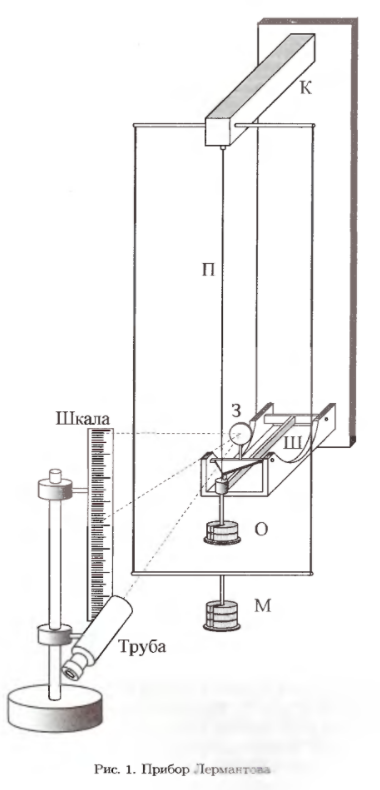
\includegraphics{131_1.jpg}}
\end{figure}

Модуль Юнга $E$ материала стержня связан со стрелой прогиба $y_{max}$ ( то есть с перемещением середины стержня) соотношением (20):

\[ E = \frac{Pl^3}{4ab^3y_{max}}.\]

Здесь $P$ -- нагрузка, вызывающая прогиб стержня, $l$ -- расстояние между призмами А и Б, $a$ и $b$ -- ширина и высота сечения стержня.

Чтобы исключить ошибки возникаюшие вследствие прогибе стола при изменении нагрузки на стержень, грузы перед началом эксперимента следует расположить на рейке над нижней полкой опорной стойки.

Формула (20) была выведена при условиях, что, во-первых, ребра опореых призм А и Б находятся на одной горизонтали (высоте и , во-вторых, сила $P$ приложена точно посередине балки.

\begin{center} 
\section{Задание}
\end{center}

\center{\textbf{Определение модуля Юнга по измерениям изгиба палки (рис.2)}}

\begin{figure}[h]
\center{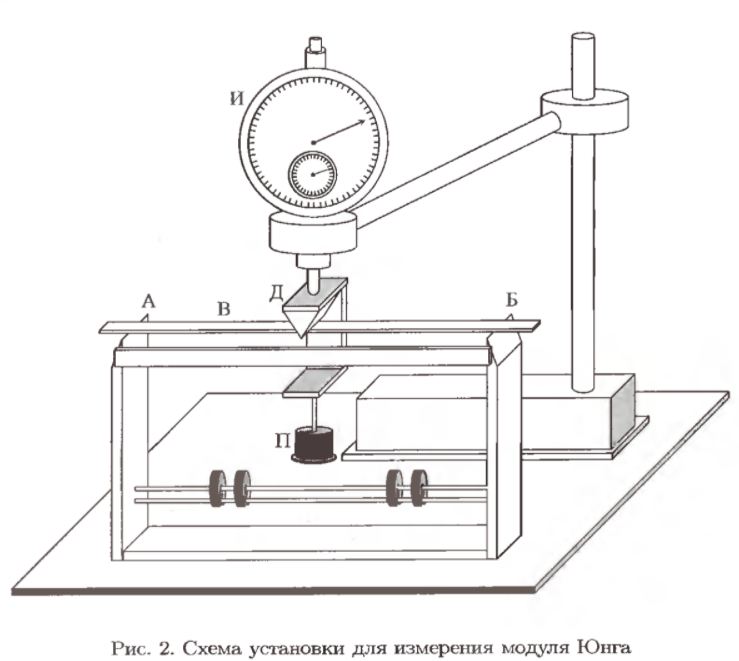
\includegraphics{131_2.jpg}}
\end{figure}


\subsection{Расстояние между ребрами}

Измерим расстояние между ребрами призм А и Б.

\begin{enumerate}
\item Измеряем $l_{ab}$ см.
\end{enumerate}

\subsection{Размеры балки(стержня)}

Определим ширину и толщину балки (стержня). Для этого измерим указанные параметры не менее чем в десяти различных местах. По ним вычислите средние значения, которые будут использованы в дальнейших расчетах.

\begin{enumerate}
\item Определяем ширину и толщину стержней). 
\end{enumerate}

\subsection{Зависимости стрелы прогиба $y_{max}$}

Исследуемую балку положим на стойку. Установим индикатор в центре балки и снимим зависимость стрелы прогиба $y_{max}$ от величины нагрузки $P$. Измерения будем проделывать при возрастании и убывании нагрузки. Проверим, возвращается ли балка в первоначальное положение после снятия нагрузки.

\begin{enumerate}
\item Кладем балку так, чтобы Д было в середине и снимаем зависимость $y_{max}$ от P. Для этого смещаем Д на 2-3 мм в сторону и сравниваем с положением в середине: угол наклона примерно один и тот же.
\end{enumerate}

\subsection{Исследования существенности зависимости результата от положения точки приложения изгибающей силы $P$}


Проведем исследования существенности зависимости результата от положения точки приложения изгибающей силы $P$. Для этого сместим призму Д на 2-3 мм от точки, принятой за середину балки, а вновь измерим стрелу прогиба. Эту величину сравним с результатом, полученным при положении призмы Д посередины балки.


\subsection{Противоположная сторона}

Перевернем балку таким образом, чтобы при нагружении она изгибалась в противоположную сторону, и повторим измерения. Сравним результаты с предыдущим.

\begin{enumerate}
\item Поворачиваем балку на 180 градусов вокруг горизонтальной оси и проделываем то же, что и в пункте 3. Сравниваем с пунктом 3:  угол наклона примерно один и тот же.  
\item Аналогично для 2-3 балок из дерева и 1 из метала. 
\item Для каждого образца строим графики при увеличении и уменьшении нагрузки.
\end{enumerate}

\subsection{Другие балки}

Аналогичные измерения проводим для 2-3 балок, изготовленных из дерева, и одной металлической.

\begin{enumerate}
\item Все данные записываем в таблицу. 
\end{enumerate}

\subsection{Построение график}

Для каждого образца построим график <<нагрузка--прогиб>> при увеличении и уменьшении нагрузки. По наклону графиков определим среднее значение модулей Юнга.

\begin{enumerate}
\item По наклону графиков определяем средние значения модулей Юнга по формуле:
\[E = \dfrac{Pl^3}{4ab^3y_{max}}\]
\end{enumerate}



\subsection{Оценка погрешностей}

Оценим погрешность результатов измерений и сравним полученные модули Юнга с соответствующими табличными значениями:


\[\sigma_E = \sqrt{3 \left( \dfrac{\sigma_{l}}{l} \right)^2 + \left( \dfrac{\sigma_{P/y_{max}}}{P/y_{max}} \right)^2 + \left( \dfrac{\sigma_{a}}{a} \right)^2 + 3 \left( \dfrac{\sigma_{b}}{b} \right)^2}\]

\section{Вывод}

Мы экспериментально получили зависимость между напряжением и деформацией (Закон Гука) для двух простейших напряженных состояний упругих тел: одноосного растяжения и чистого изгиба. Так же смогли по полученным результатам вычислить модуль Юнга.

\end{document}